\documentclass{ethz_report}
\usepackage{listings}
\usepackage{color}
\usepackage{caption}
\usepackage{subcaption}


\definecolor{codegreen}{rgb}{0,0.6,0}
\definecolor{codegray}{rgb}{0.5,0.5,0.5}
\definecolor{codepurple}{rgb}{0.58,0,0.82}
\definecolor{backcolour}{rgb}{1,1,1}

\lstdefinestyle{mystyle}{
    backgroundcolor=\color{backcolour},
    commentstyle=\color{codegreen},
    keywordstyle=\color{magenta},
    numberstyle=\tiny\color{codegray},
    stringstyle=\color{codepurple},
    basicstyle=\ttfamily,
    breakatwhitespace=false,
    breaklines=true,
    captionpos=b,
    keepspaces=true,
    numbers=left,
    numbersep=5pt,
    showspaces=false,
    showstringspaces=false,
    showtabs=false,
    tabsize=4,
    frame=lines
}
\lstset{style=mystyle}

\title{Exercise 8 - Condensation Tracker}
\subject{Computer Vision}
\author{Alberto Montes}
\email{malberto@student.ethz.ch}
\date{\today}

\begin{document}
\maketitle

\section*{Implementation}

The task consist into implement the color histogram computation. The function needs to take into account the bounding box that overlap with the frame, compute the histogram, and then normalize it to sum up 1. The implementation is on Listing~\ref{lst:color_histogram}.

\lstinputlisting[language=MATLAB, caption=color\_histogram.m, label={lst:color_histogram}]{../code/color_histogram.m}

Then to compute the propagation of particles, there are two ways of model it: no movement and constant velocity. For the first one, the particles are represented as $x$, $y$ coordinates and the matrix A is the following:

\begin{equation}
    \begin{bmatrix}
        x \\ y
    \end{bmatrix}_t = A \cdot \begin{bmatrix}
        x \\ y
    \end{bmatrix}_{t-1} + w_{t-1} = \begin{bmatrix}
        1 & 0 \\ 0 & 1
    \end{bmatrix} \cdot \begin{bmatrix}
        x \\ y
    \end{bmatrix}_{t-1}
\end{equation}

In the case the model take into account constant movement, the particles are represented as coordinates and velocities for each coordinates, and the model matrix $A$ is:

\begin{equation}
    \begin{bmatrix}
        x \\ y \\ \dot{x} \\ \dot{y}
    \end{bmatrix}_t = A \cdot \begin{bmatrix}
        x \\ y \\ \dot{x} \\ \dot{y}
    \end{bmatrix}_{t-1} + w_{t-1} = \begin{bmatrix}
        1 & 0 & 1 & 0 \\ 0 & 1 & 0 & 1 \\ 0 & 0 & 1 & 0 \\ 0 & 0 & 0 & 1
    \end{bmatrix} \cdot \begin{bmatrix}
        x \\ y \\ \dot{x} \\ \dot{y}
    \end{bmatrix}_{t-1}
\end{equation}

This computation implemented on the propagate function is on Listing~\ref{lst:propagate} where the propagation is computed and then a random noise is added.

\lstinputlisting[language=MATLAB, caption=propagate.m, label={lst:propagate}]{../code/propagate.m}

Then, the particles needs to be observed, where for each particle, the surrounding bounding box is extracted and its color histogram is computed.
Then for each particle, a weight is computed following a Gaussian and the chi squared distance of the original histogram and the one computed for each particle. The implementation is on Listing~\ref{lst:observe}.

\lstinputlisting[language=MATLAB, caption=observe.m, label={lst:observe}]{../code/observe.m}

With all the particle and its respective weights, it must be estimated the position of the object to track computing a weighted mean along all the particles coordinates and velocities to obtain an estimation for each time step.

\lstinputlisting[language=MATLAB, caption=estimate.m, label={lst:estimate}]{../code/estimate.m}

Finally a resample is performed to keep the particles with higher weight and remove the ones less probable. The algorithm of resampling is the same used on Exercise~3 about the robot localization using particle filters too. The implementation of the resampling function is on Listing~\ref{lst:resample}

\lstinputlisting[language=MATLAB, caption=resample.m, label={lst:resample}]{../code/resample.m}

\section*{Experiments}

Once the implementation is finished, is time to experiment with different videos, scenarios and parameters to see and understand the behavior of the Condensation Tracker.

\subsection*{\texttt{video1.wmv}}

With the first video, where the background is uniform and there is a moving hand, it can be seen how the condensation tracker is capable of tracking the hand until this disappear (Figure~\ref{fig:tracking_video1}).

The tracker is capable to follow the hand but with some limitations on the trajectory predictions. As it is initialize with only some fingers on the view, then the observations tent to give a high score at any part of the hand or arm so the trajectory predicted is not smooth. Also remark that when the hand completely disappear the frame, the position prediction tent to go to the bottom left corner, where the histogram is more similar to the initial one.

\begin{figure}[H]
    \centering
    \begin{subfigure}[b]{.25\textwidth}
        \centering
        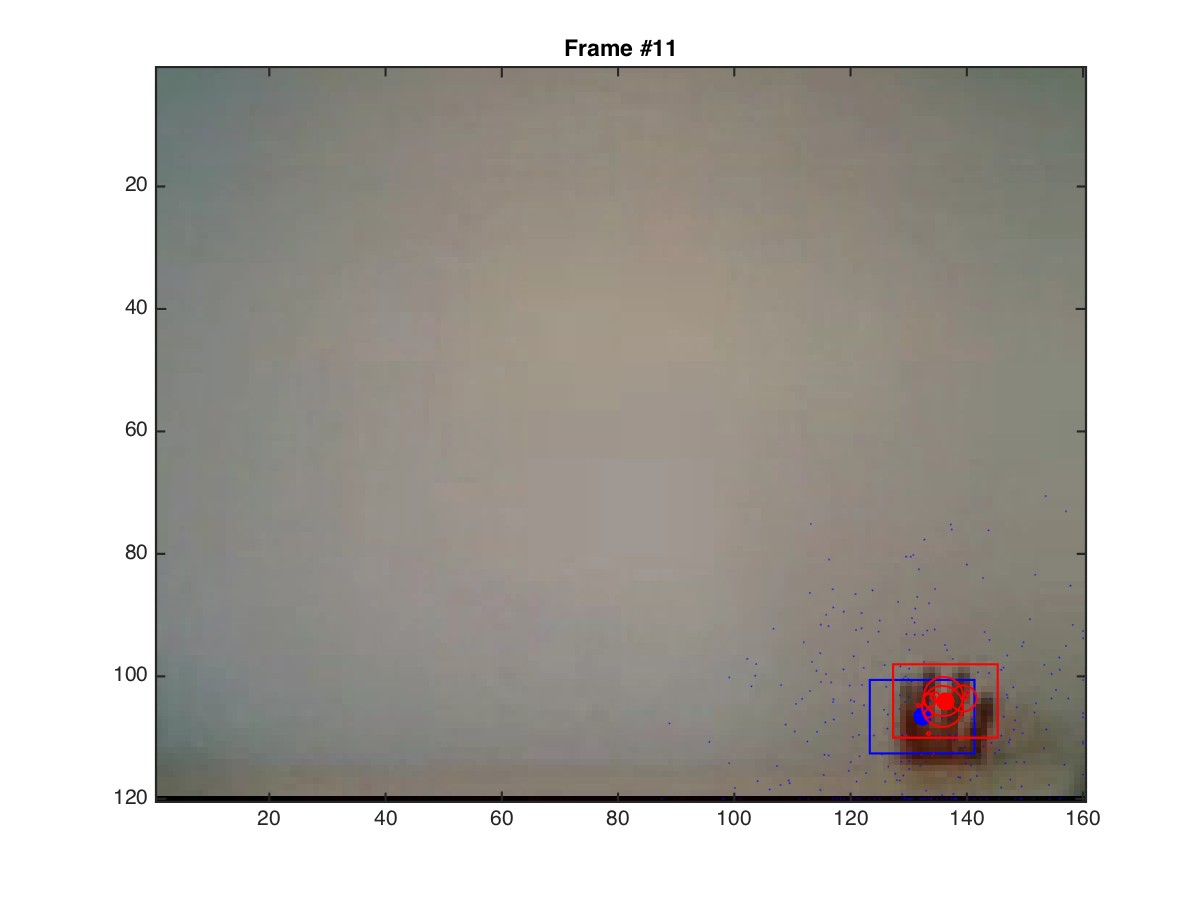
\includegraphics[width=1\linewidth]{images/video1_1}
    \end{subfigure}%
    \begin{subfigure}[b]{.25\textwidth}
        \centering
        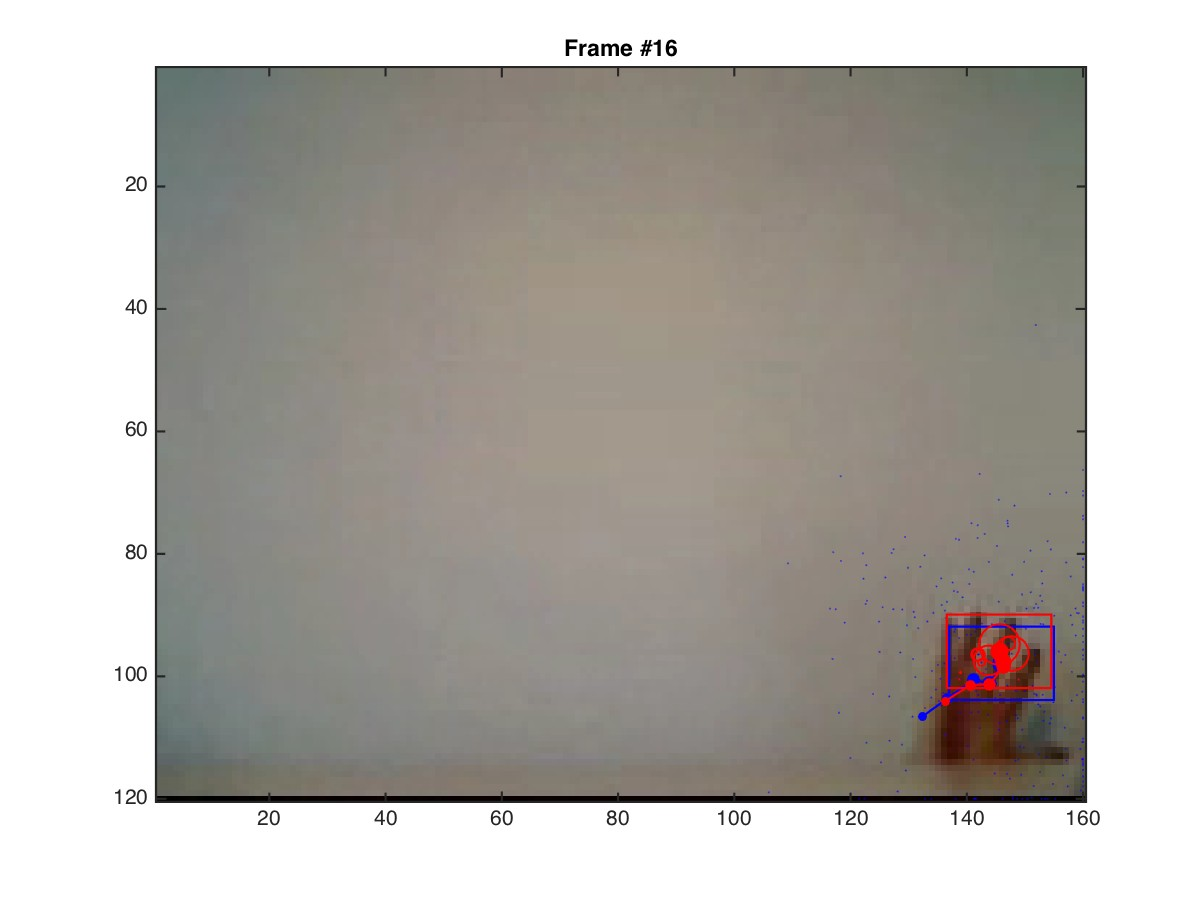
\includegraphics[width=1\linewidth]{images/video1_6}
    \end{subfigure}%
    \begin{subfigure}[b]{.25\textwidth}
        \centering
        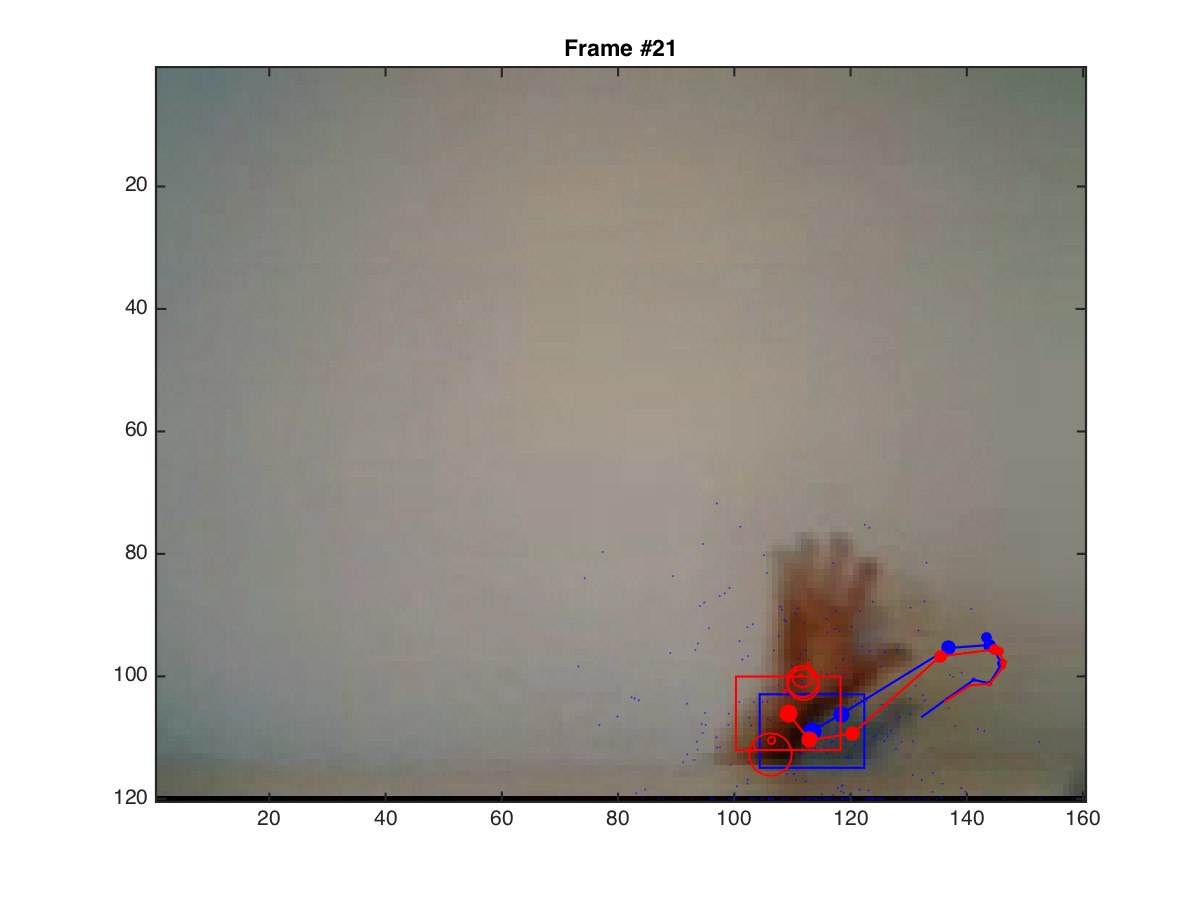
\includegraphics[width=1\linewidth]{images/video1_11}
    \end{subfigure}%
    \begin{subfigure}[b]{.25\textwidth}
        \centering
        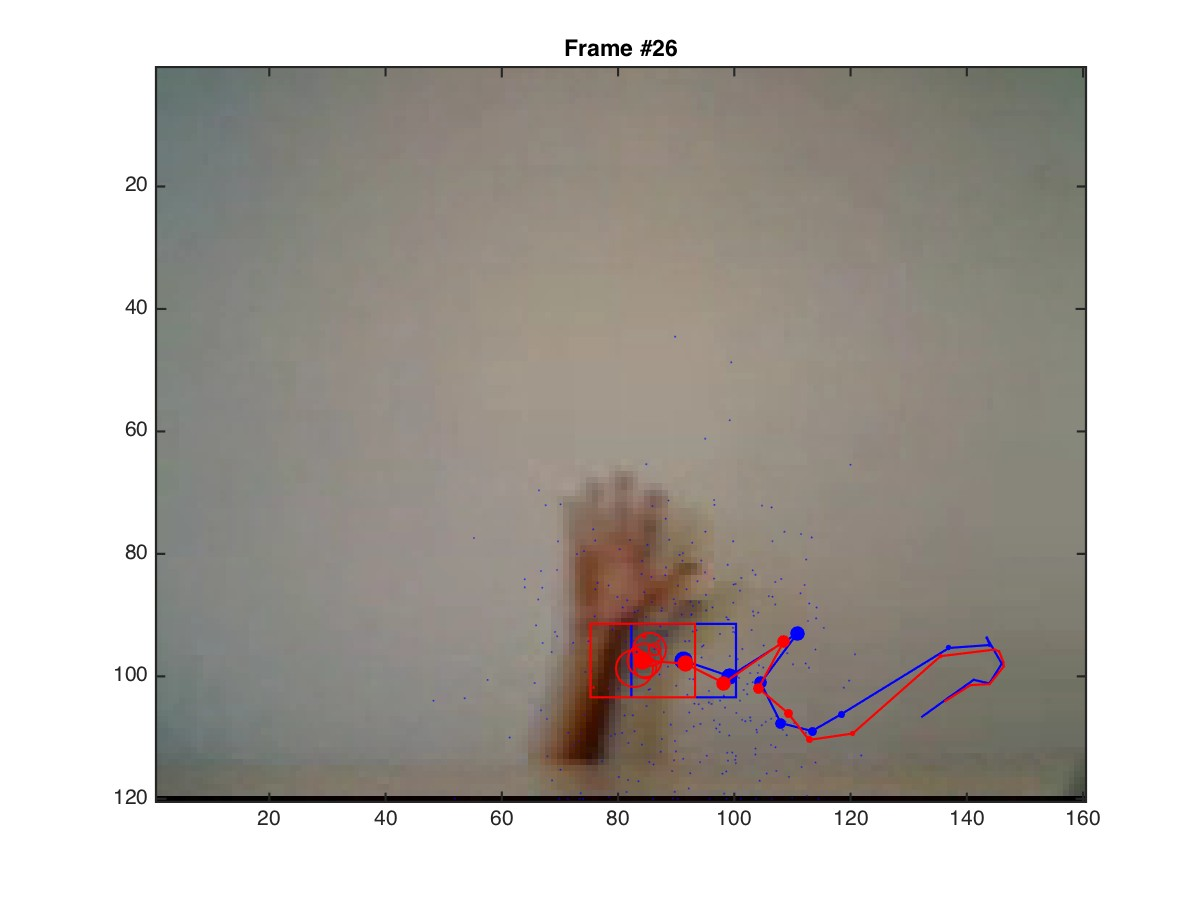
\includegraphics[width=1\linewidth]{images/video1_16}
    \end{subfigure}
    \begin{subfigure}[b]{.25\textwidth}
        \centering
        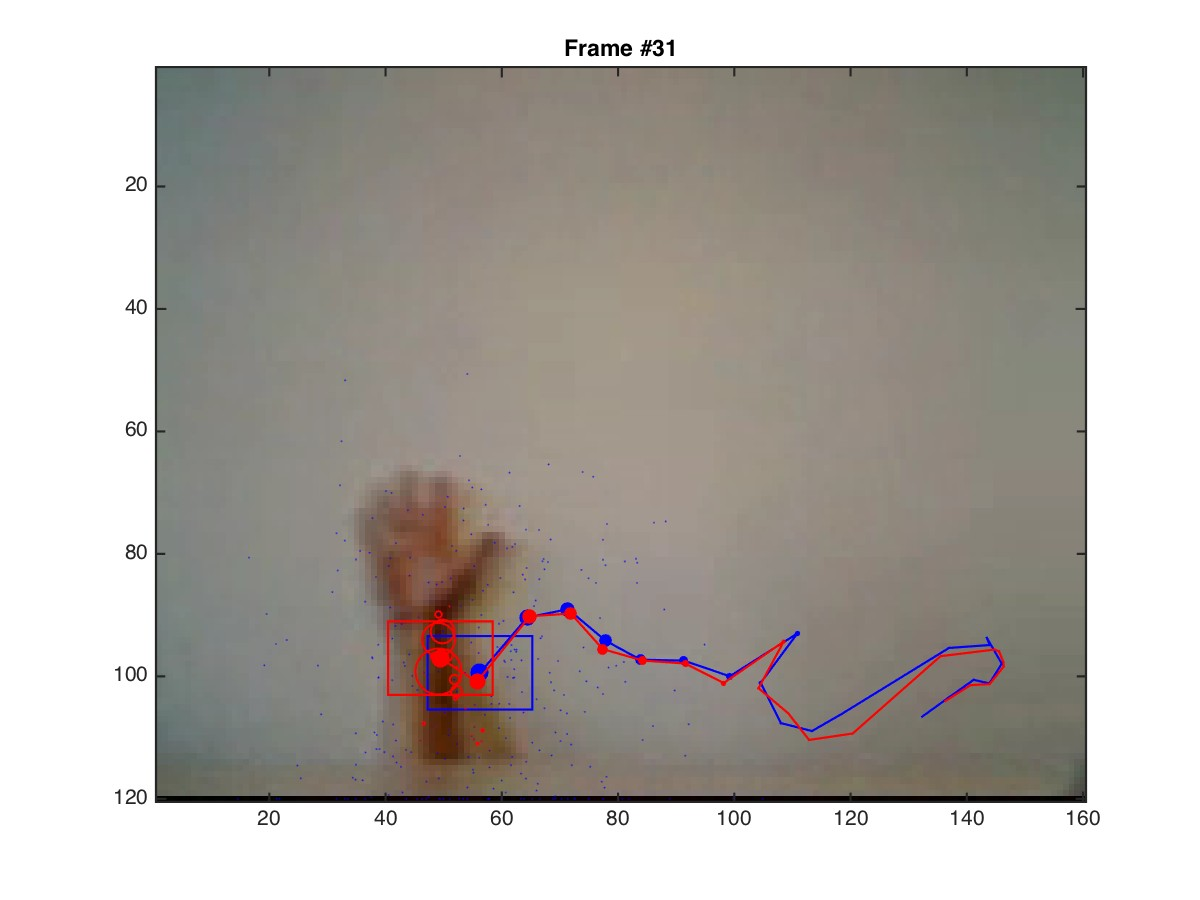
\includegraphics[width=1\linewidth]{images/video1_21}
    \end{subfigure}%
    \begin{subfigure}[b]{.25\textwidth}
        \centering
        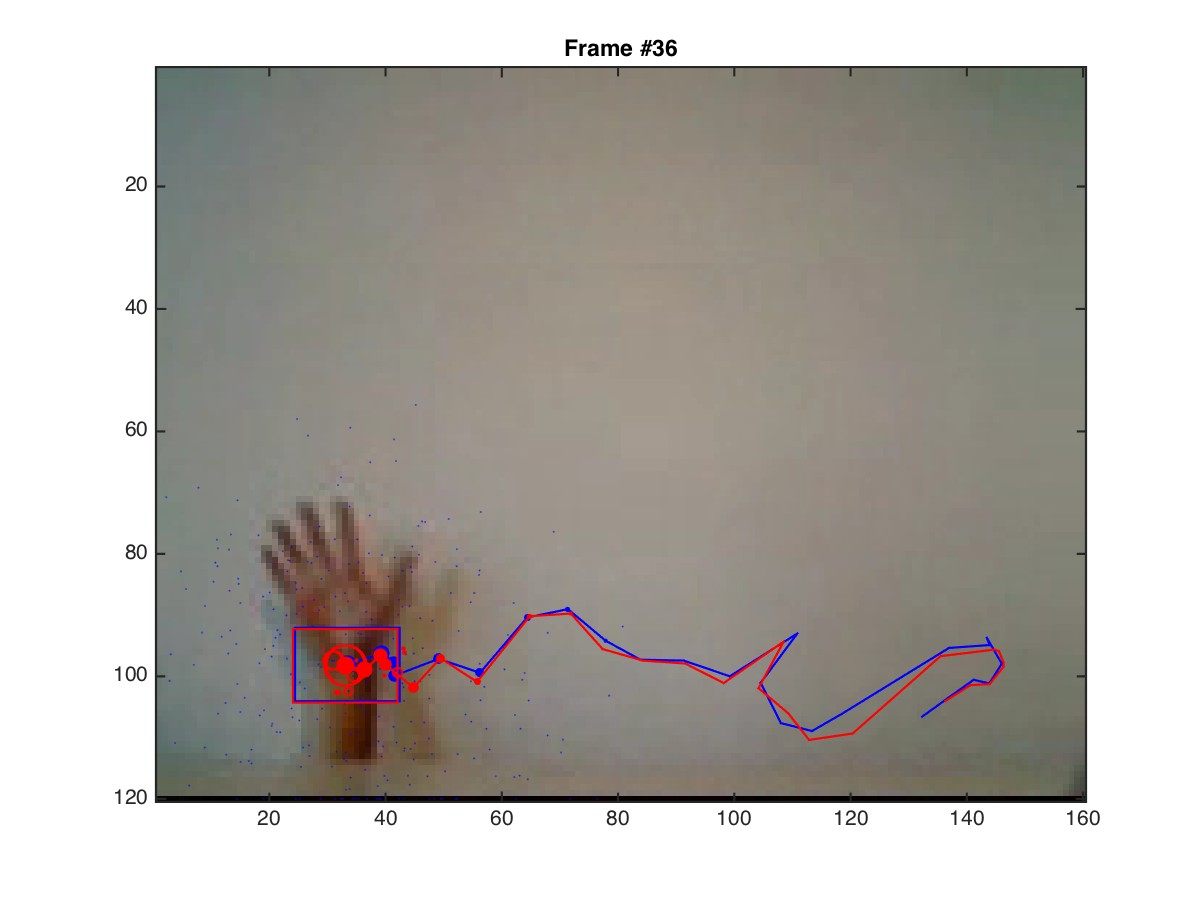
\includegraphics[width=1\linewidth]{images/video1_26}
    \end{subfigure}%
    \begin{subfigure}[b]{.25\textwidth}
        \centering
        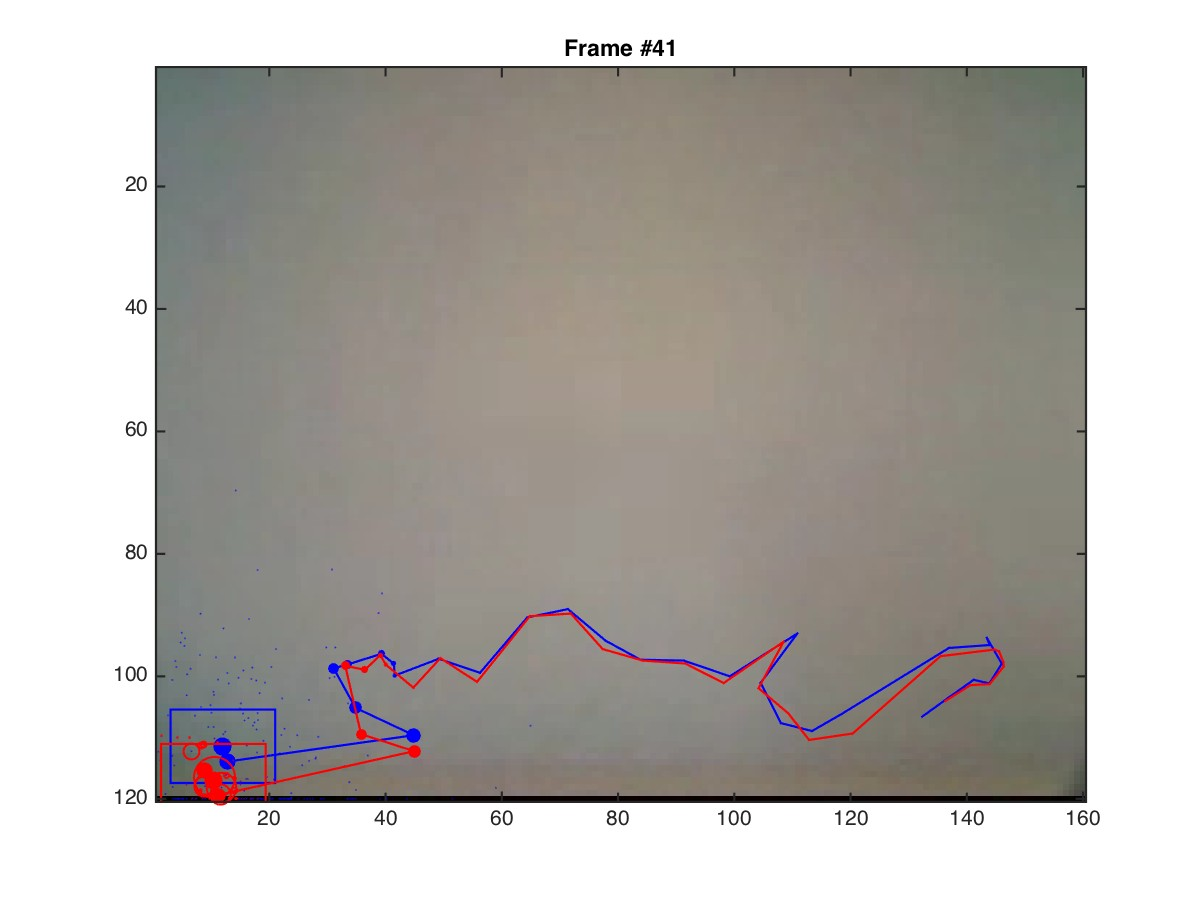
\includegraphics[width=1\linewidth]{images/video1_31}
    \end{subfigure}
    \caption{Tracking of the hand at the first video using the implemented Condensation Tracker}
    \label{fig:tracking_video1}
\end{figure}

\subsection*{\texttt{video2.wmv}}

First, with the default parameters, on Figure~\ref{fig:tracking_video1} there is the tracking for \texttt{vide2.wmv}. It can be seen how the tracker has been able to follow the object even whit an occlusion.

\begin{figure}[H]
    \centering
    \begin{subfigure}[b]{.25\textwidth}
        \centering
        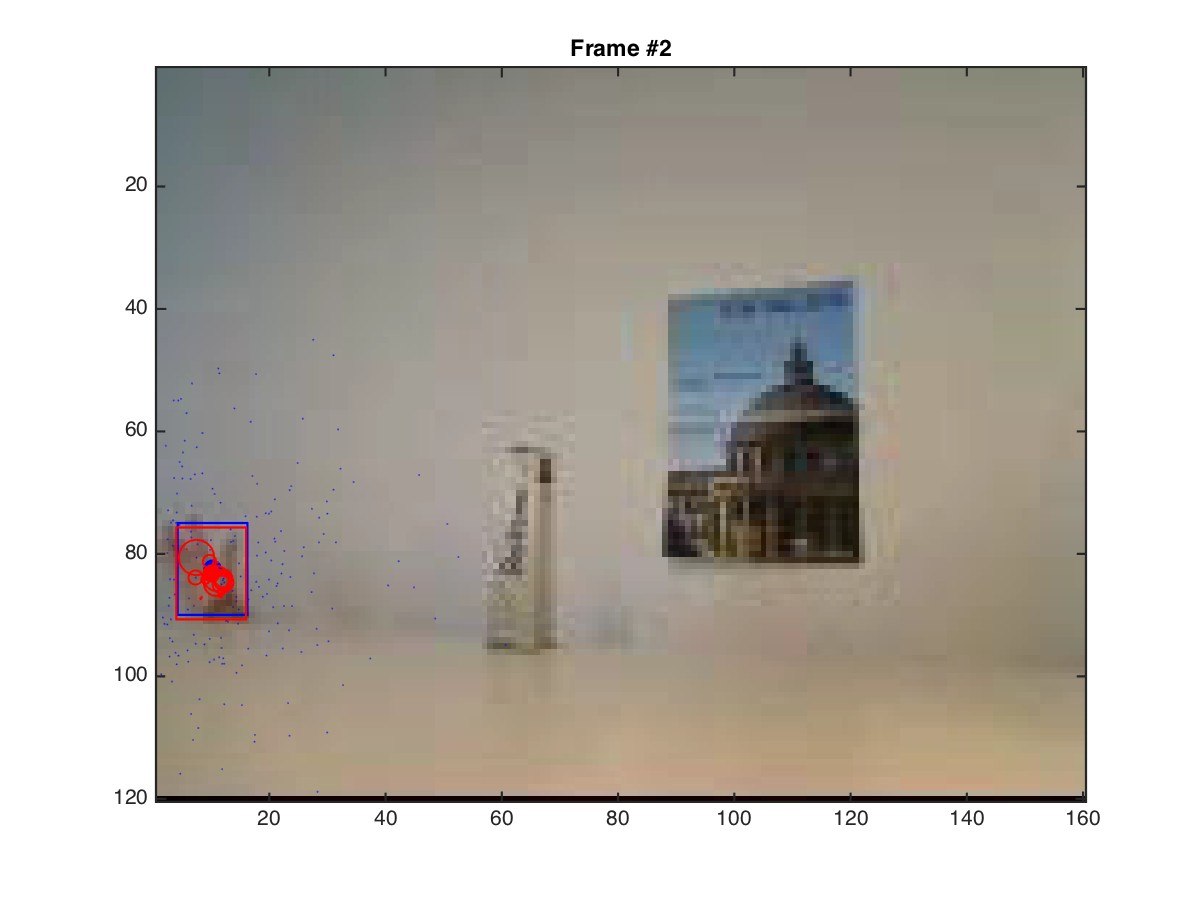
\includegraphics[width=1\linewidth]{images/video2__1}
    \end{subfigure}%
    \begin{subfigure}[b]{.25\textwidth}
        \centering
        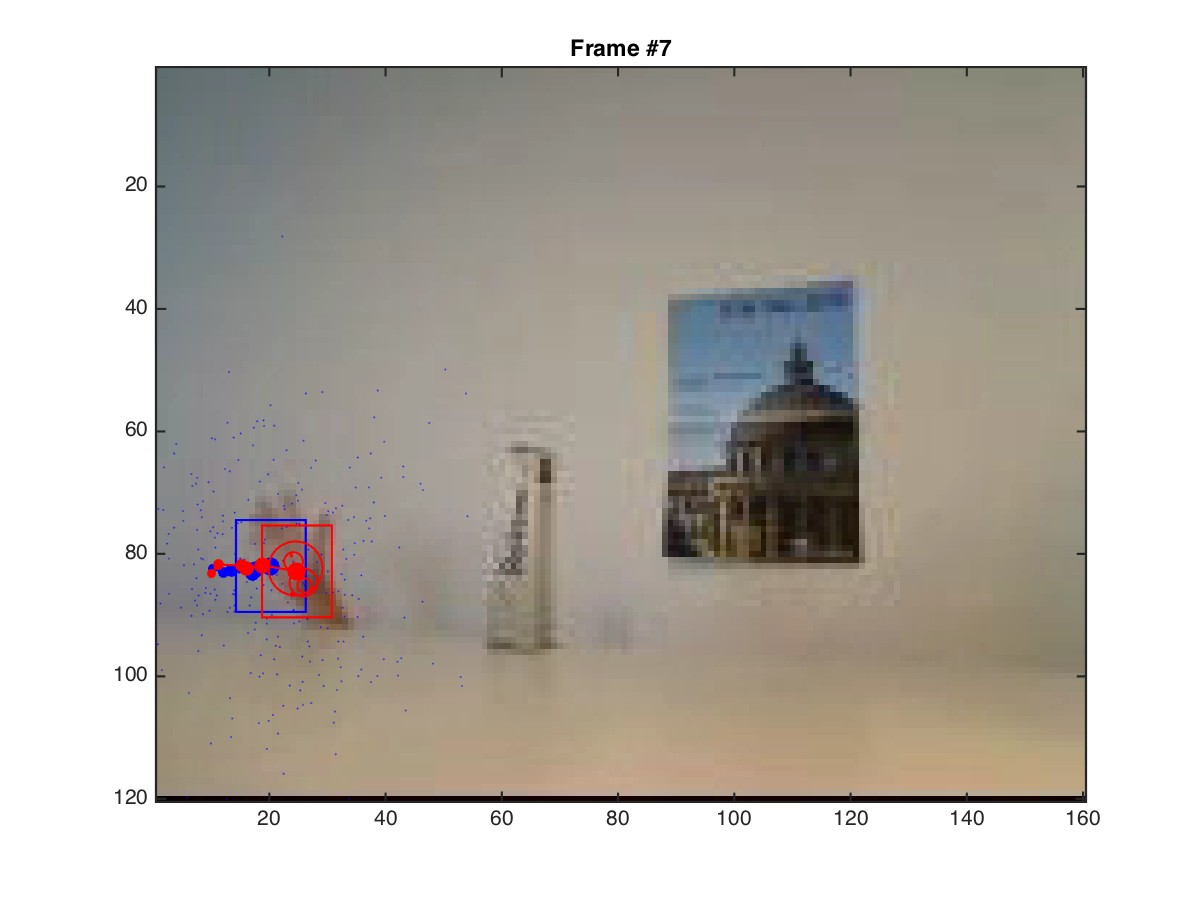
\includegraphics[width=1\linewidth]{images/video2__6}
    \end{subfigure}%
    \begin{subfigure}[b]{.25\textwidth}
        \centering
        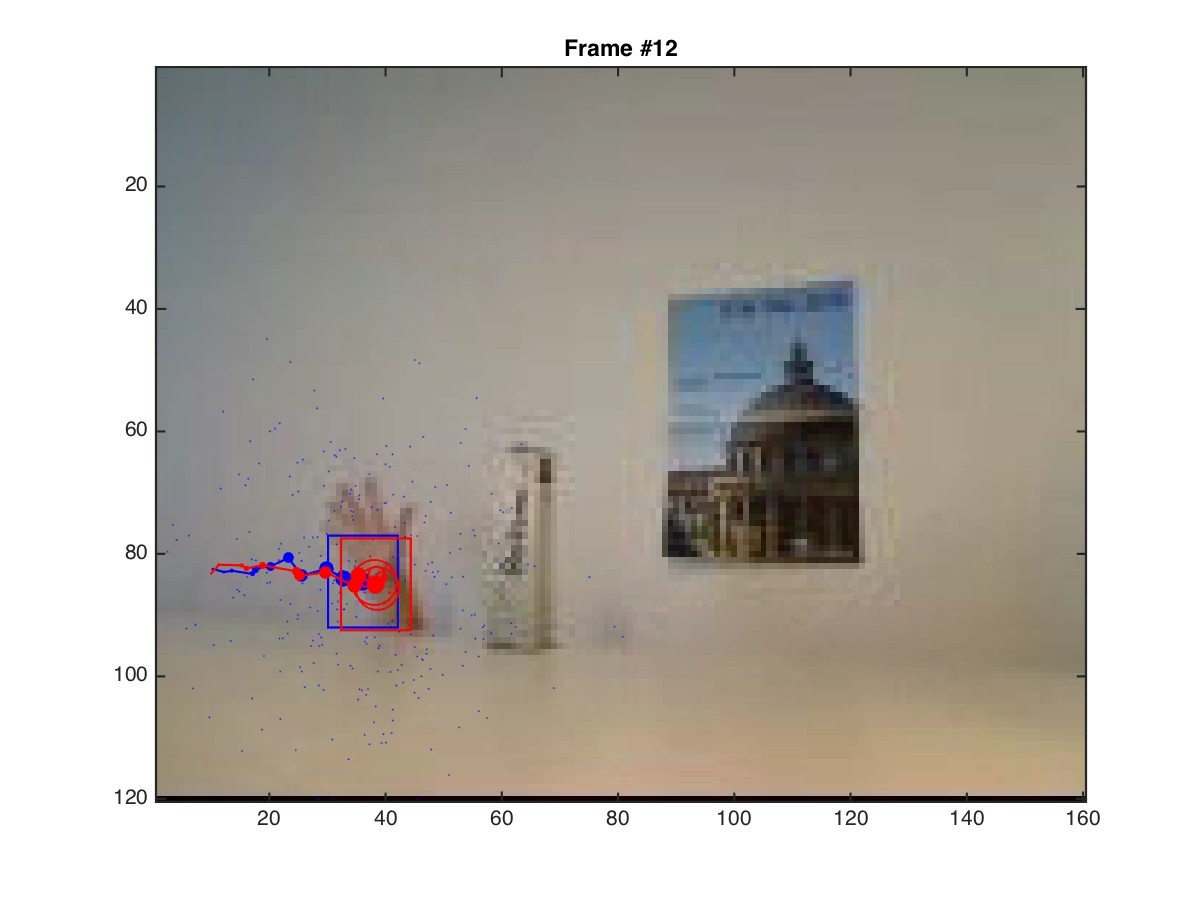
\includegraphics[width=1\linewidth]{images/video2__11}
    \end{subfigure}%
    \begin{subfigure}[b]{.25\textwidth}
        \centering
        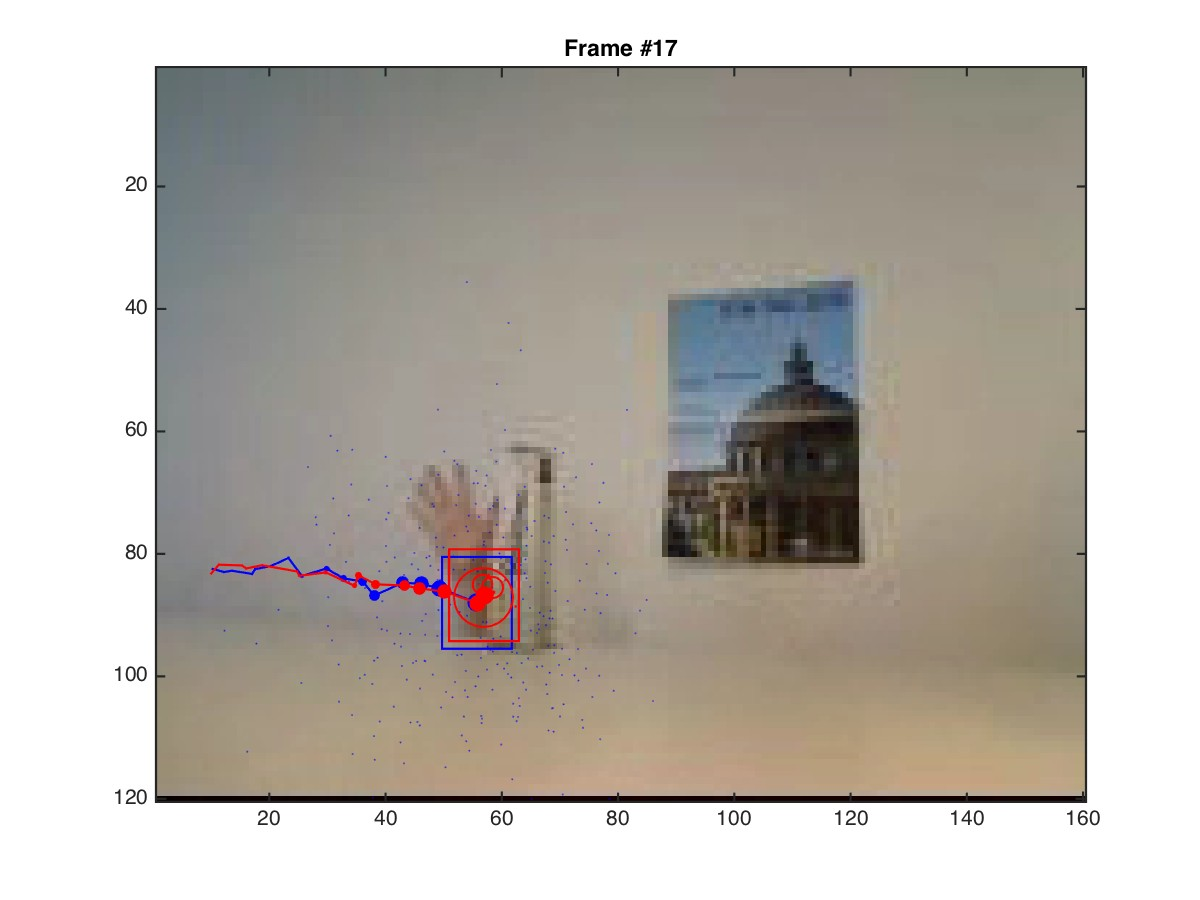
\includegraphics[width=1\linewidth]{images/video2__16}
    \end{subfigure}
    \begin{subfigure}[b]{.25\textwidth}
        \centering
        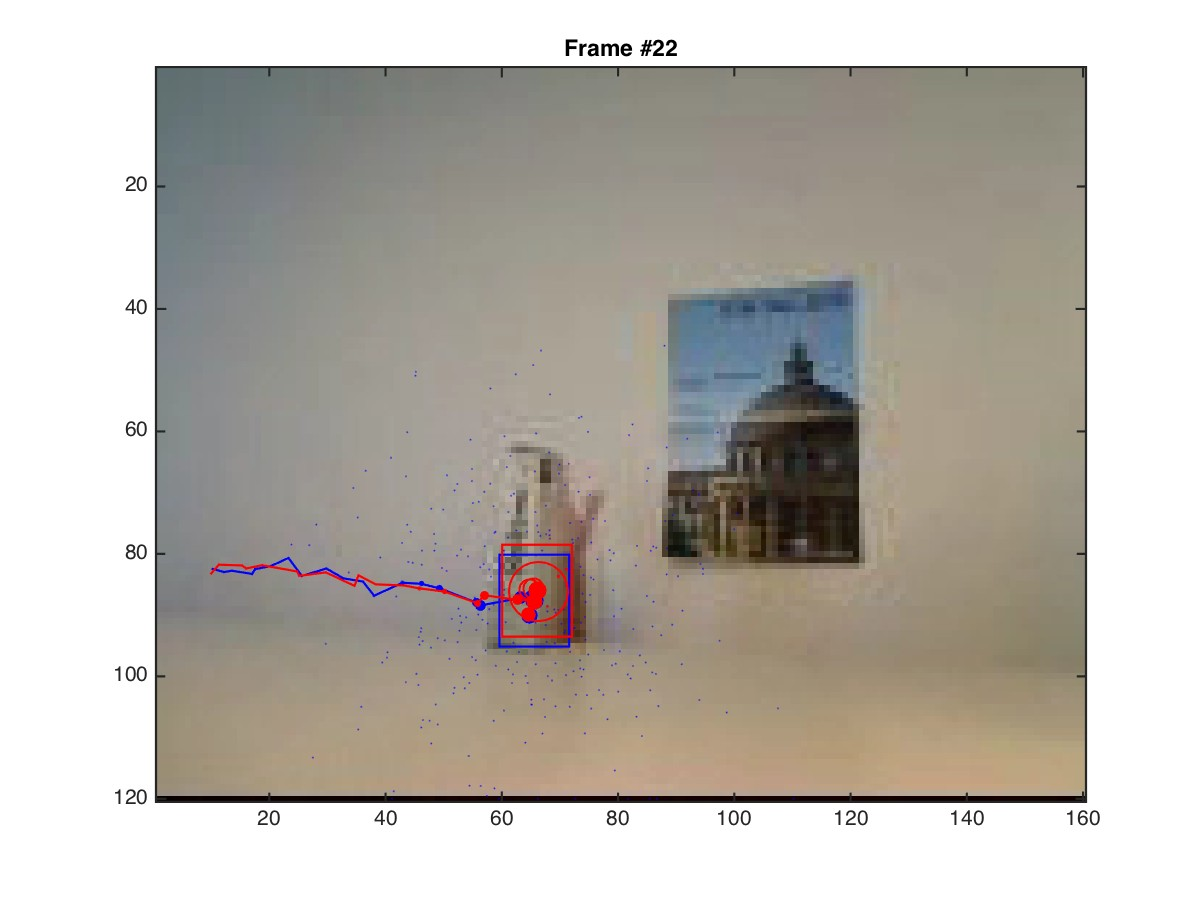
\includegraphics[width=1\linewidth]{images/video2__21}
    \end{subfigure}%
    \begin{subfigure}[b]{.25\textwidth}
        \centering
        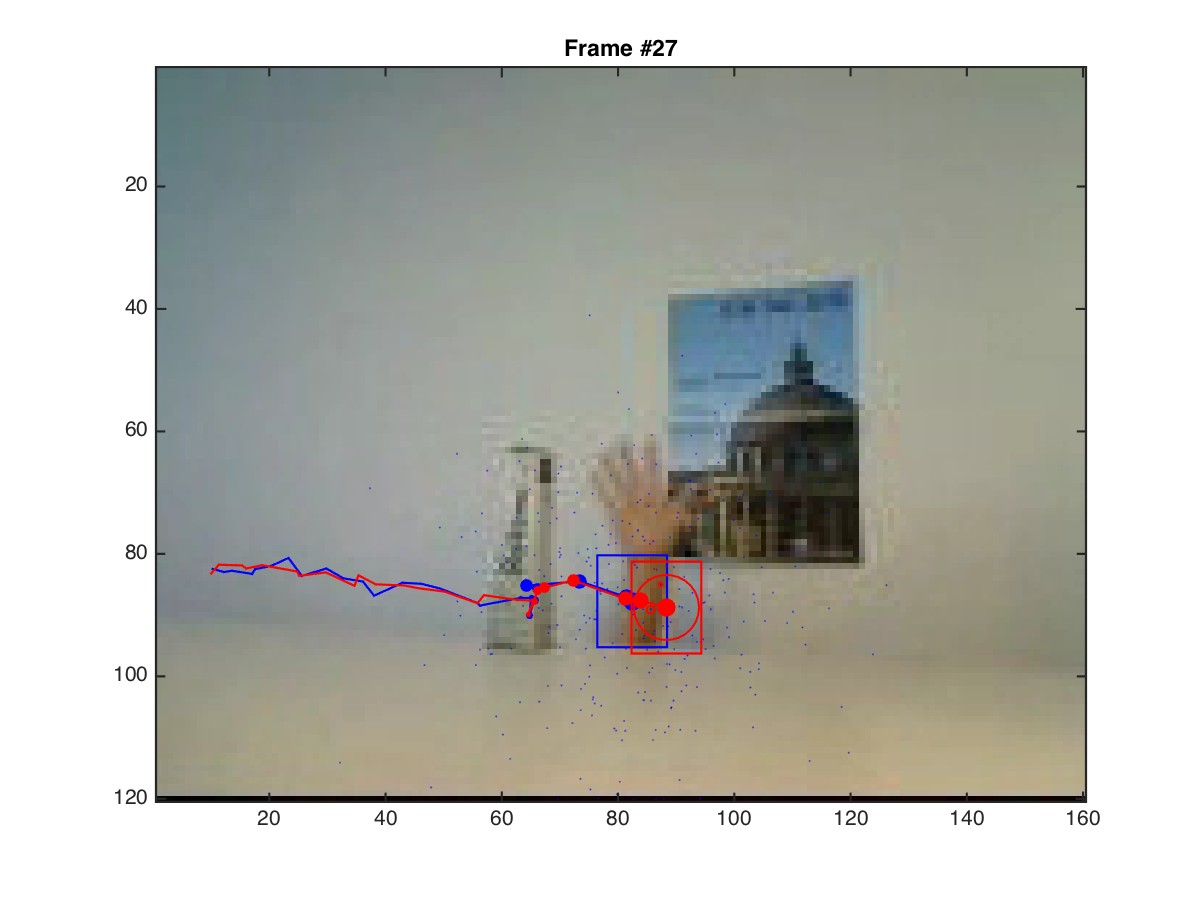
\includegraphics[width=1\linewidth]{images/video2__26}
    \end{subfigure}%
    \begin{subfigure}[b]{.25\textwidth}
        \centering
        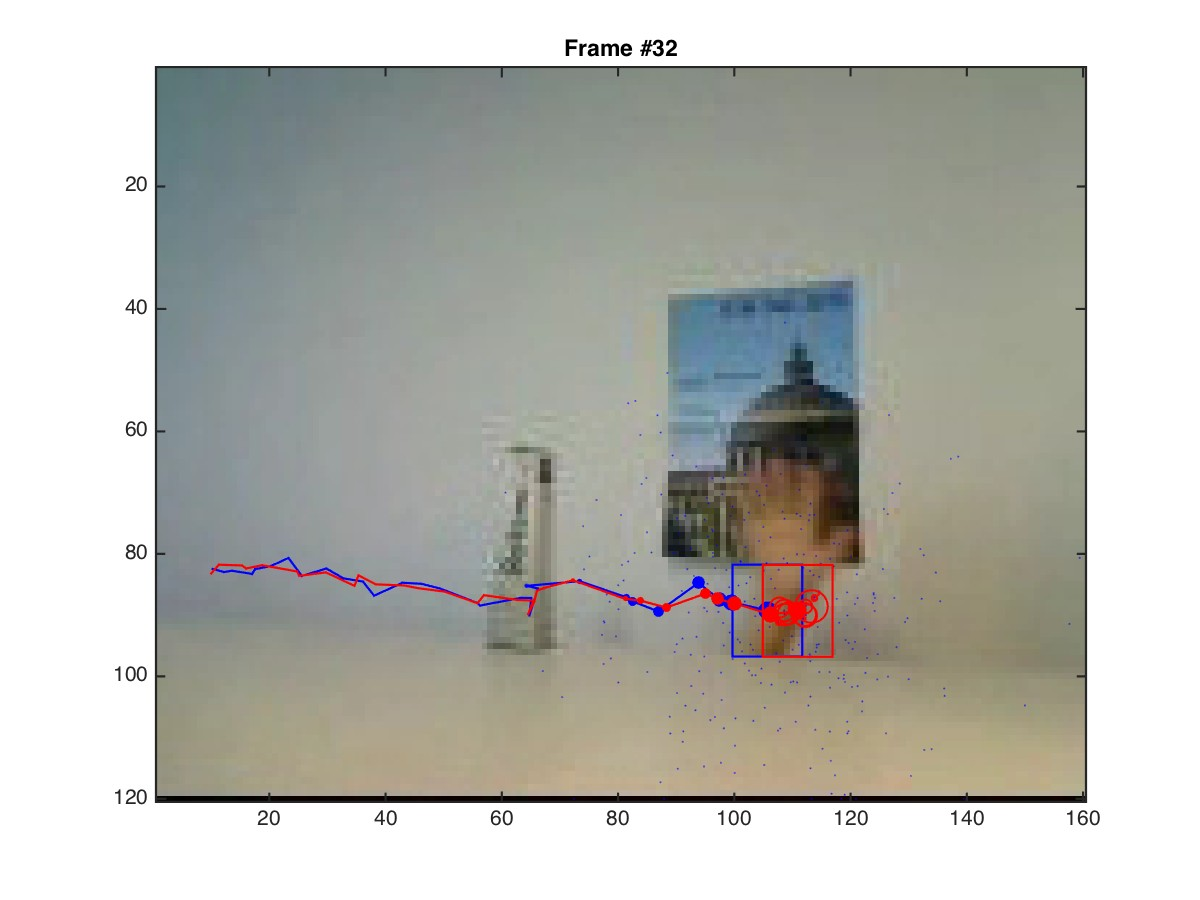
\includegraphics[width=1\linewidth]{images/video2__31}
    \end{subfigure}%
    \begin{subfigure}[b]{.25\textwidth}
        \centering
        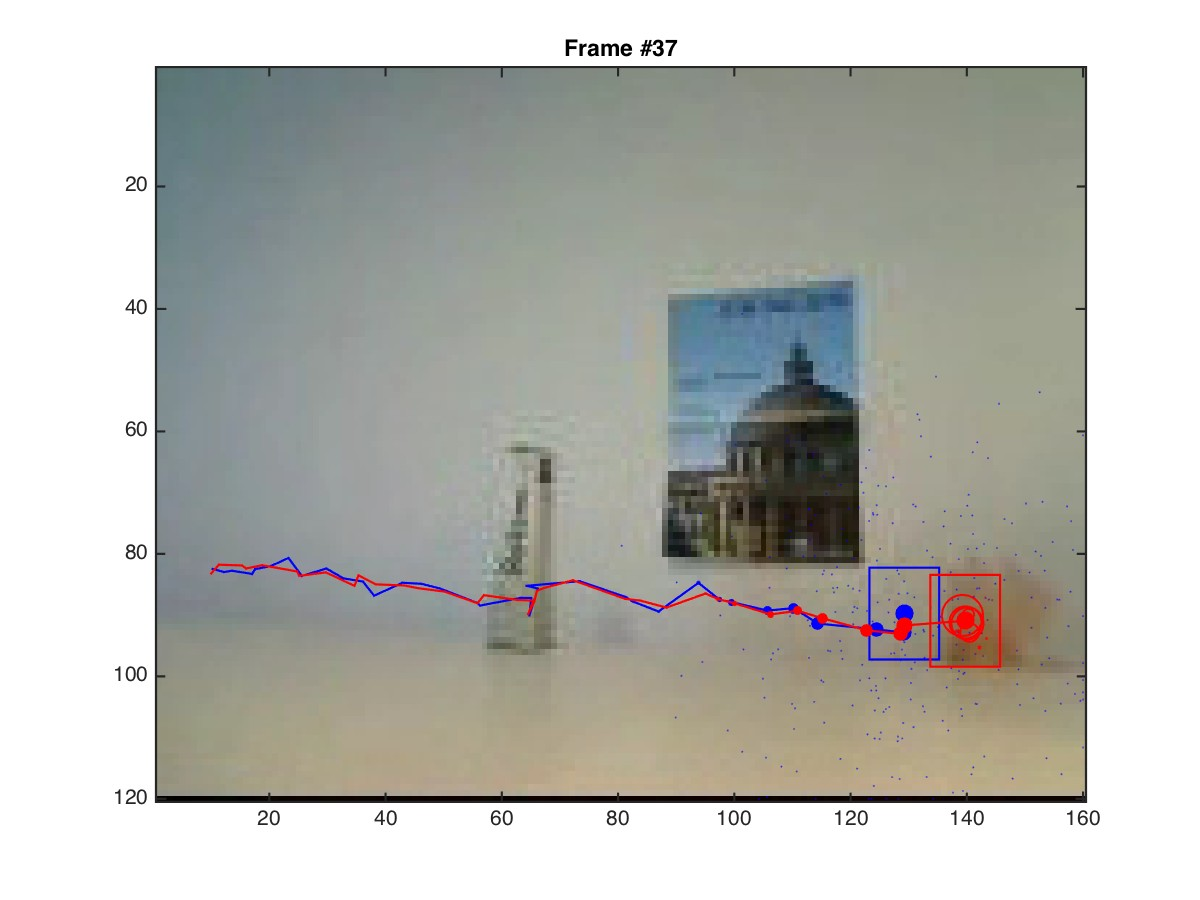
\includegraphics[width=1\linewidth]{images/video2__36}
    \end{subfigure}
    \caption{Tracking of the hand at the second video using the implemented Condensation Tracker}
    \label{fig:tracking_video2}
\end{figure}

\subsubsection*{Effect of the model}

In order to study the performance of the tracker depending on its parameters, first, the constant velocity model is tested.
The tracking is on Figure~\ref{fig:tracking_video2_model} where it can be seen how, as the initial velocity was set wit $v_0 = [ 1, 10 ]^T$, the prior probability distribution tent to predict in a lower position in the vertical axis. 
But thanks to the observations, and the enough dispersion of the particles, the posterior probability perfectly tracks the object even when this is occluded.

\begin{figure}[H]
    \centering
    \begin{subfigure}[b]{.25\textwidth}
        \centering
        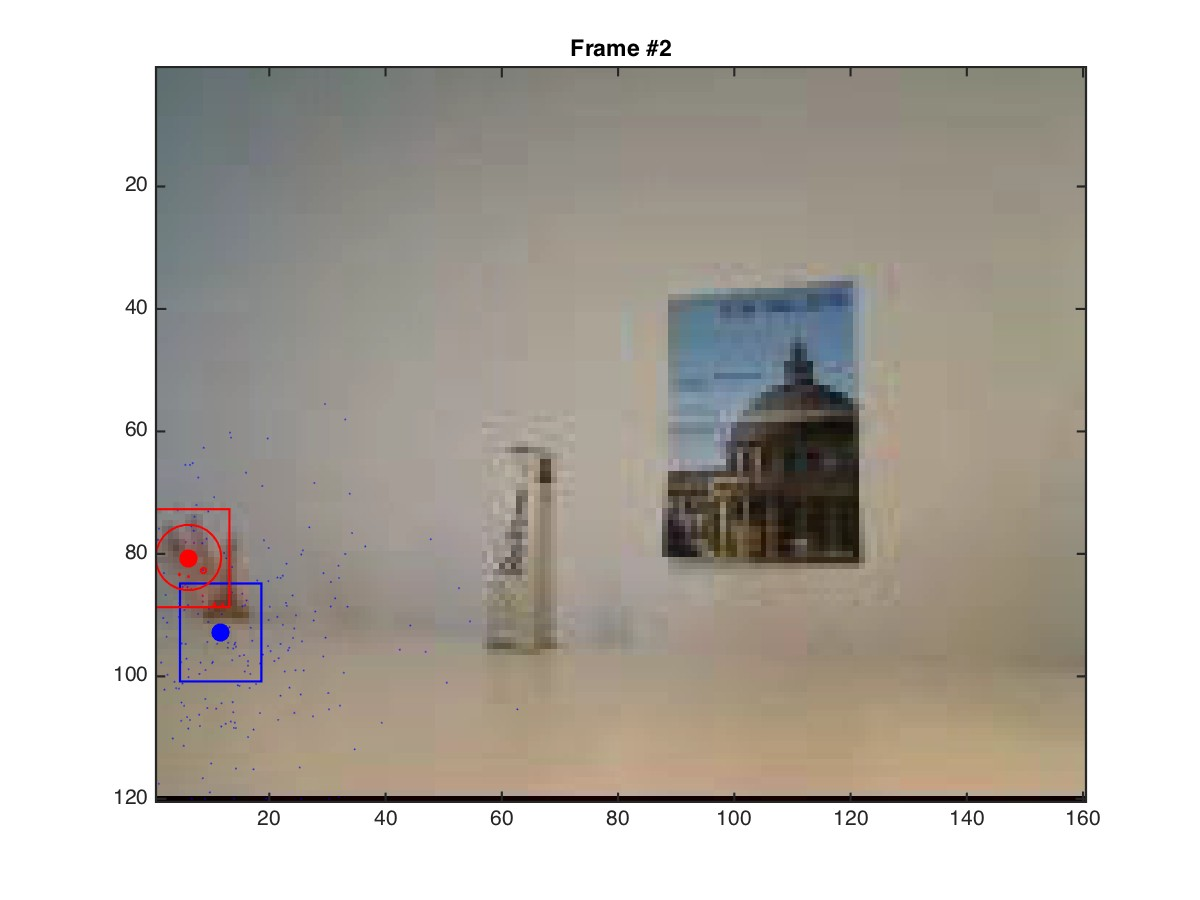
\includegraphics[width=1\linewidth]{images/video2_model_1}
    \end{subfigure}%
    \begin{subfigure}[b]{.25\textwidth}
        \centering
        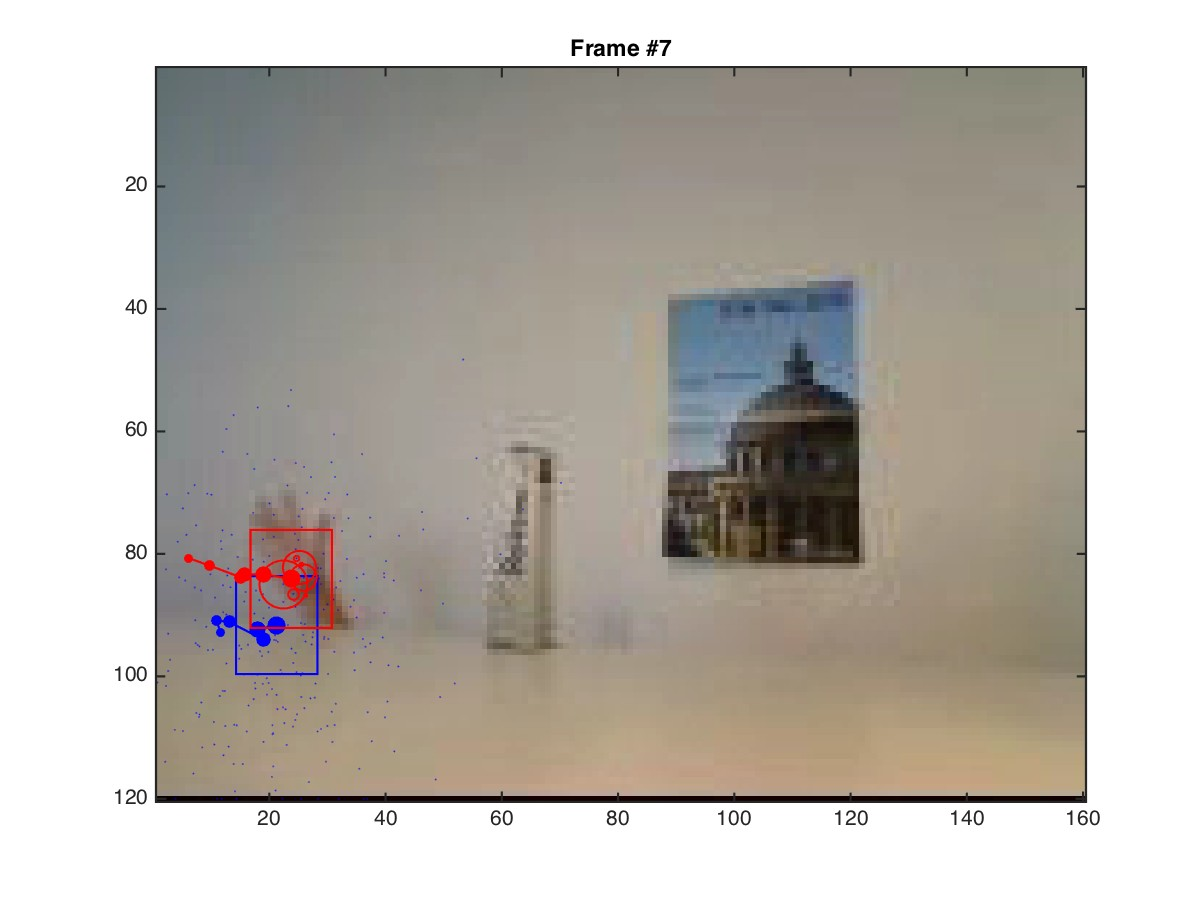
\includegraphics[width=1\linewidth]{images/video2_model_6}
    \end{subfigure}%
    \begin{subfigure}[b]{.25\textwidth}
        \centering
        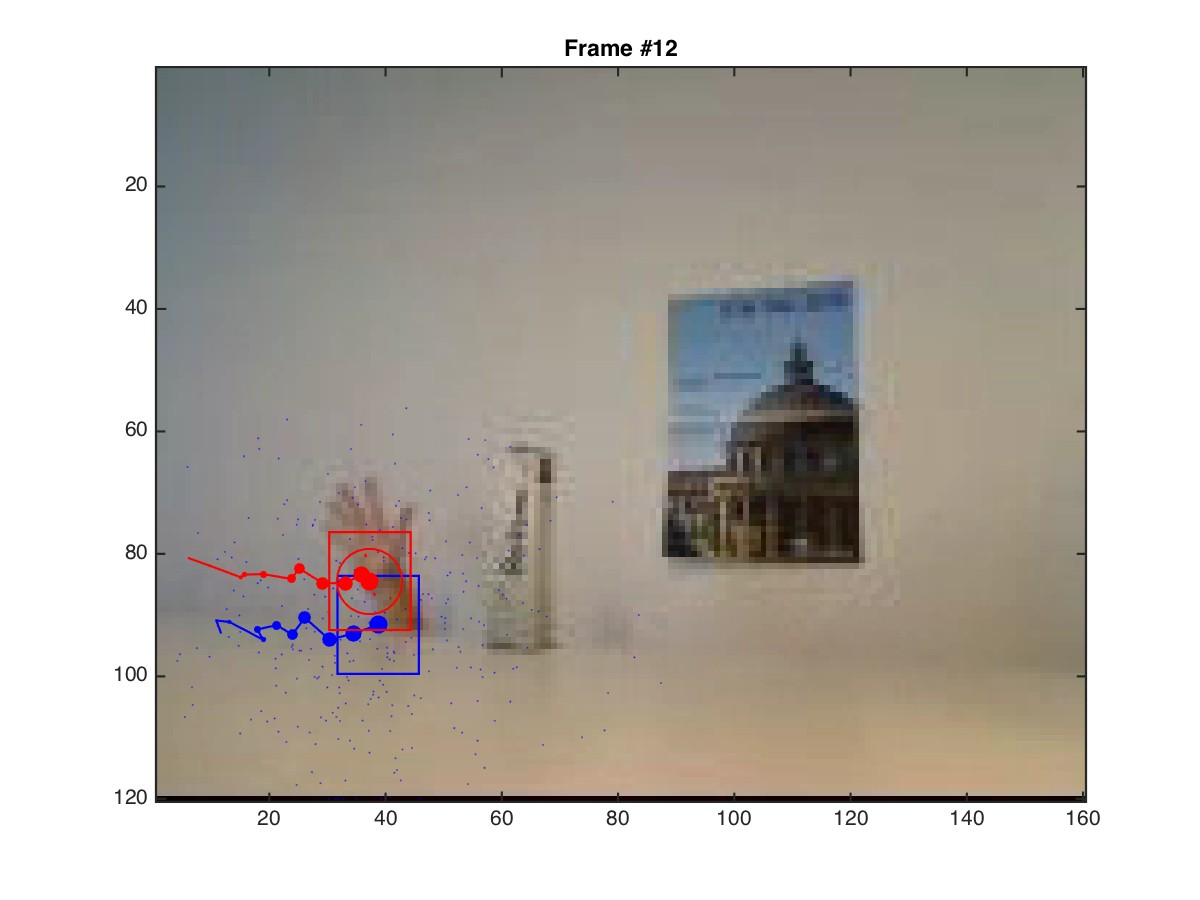
\includegraphics[width=1\linewidth]{images/video2_model_11}
    \end{subfigure}%
    \begin{subfigure}[b]{.25\textwidth}
        \centering
        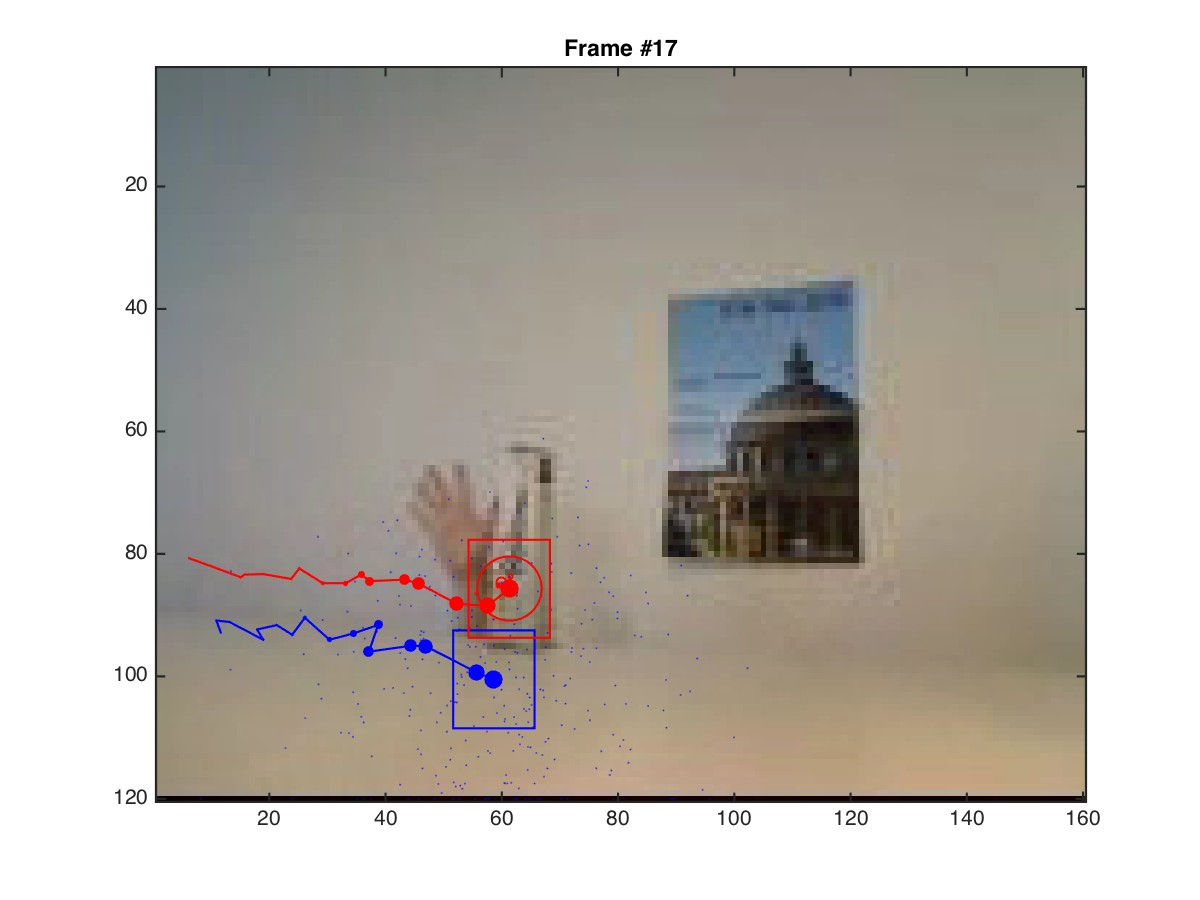
\includegraphics[width=1\linewidth]{images/video2_model_16}
    \end{subfigure}
    \begin{subfigure}[b]{.25\textwidth}
        \centering
        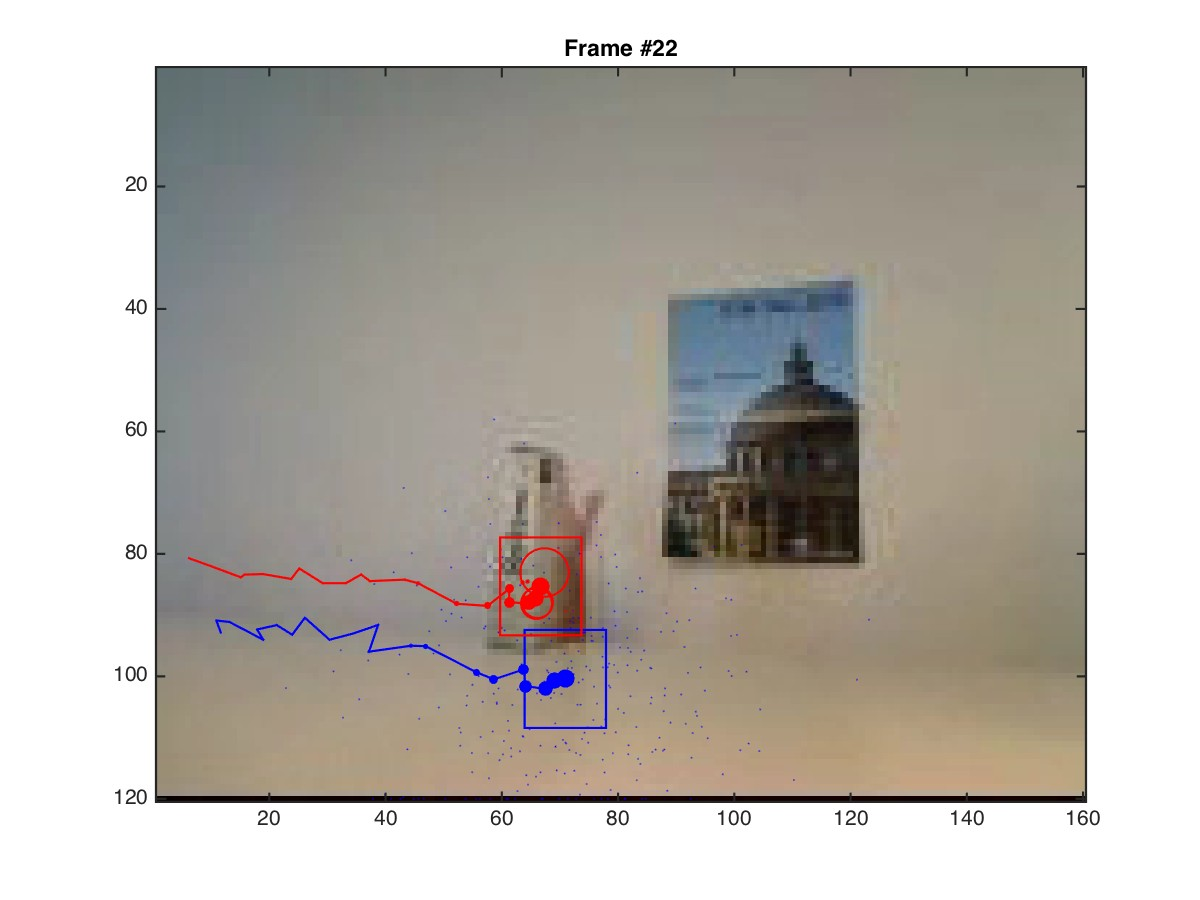
\includegraphics[width=1\linewidth]{images/video2_model_21}
    \end{subfigure}%
    \begin{subfigure}[b]{.25\textwidth}
        \centering
        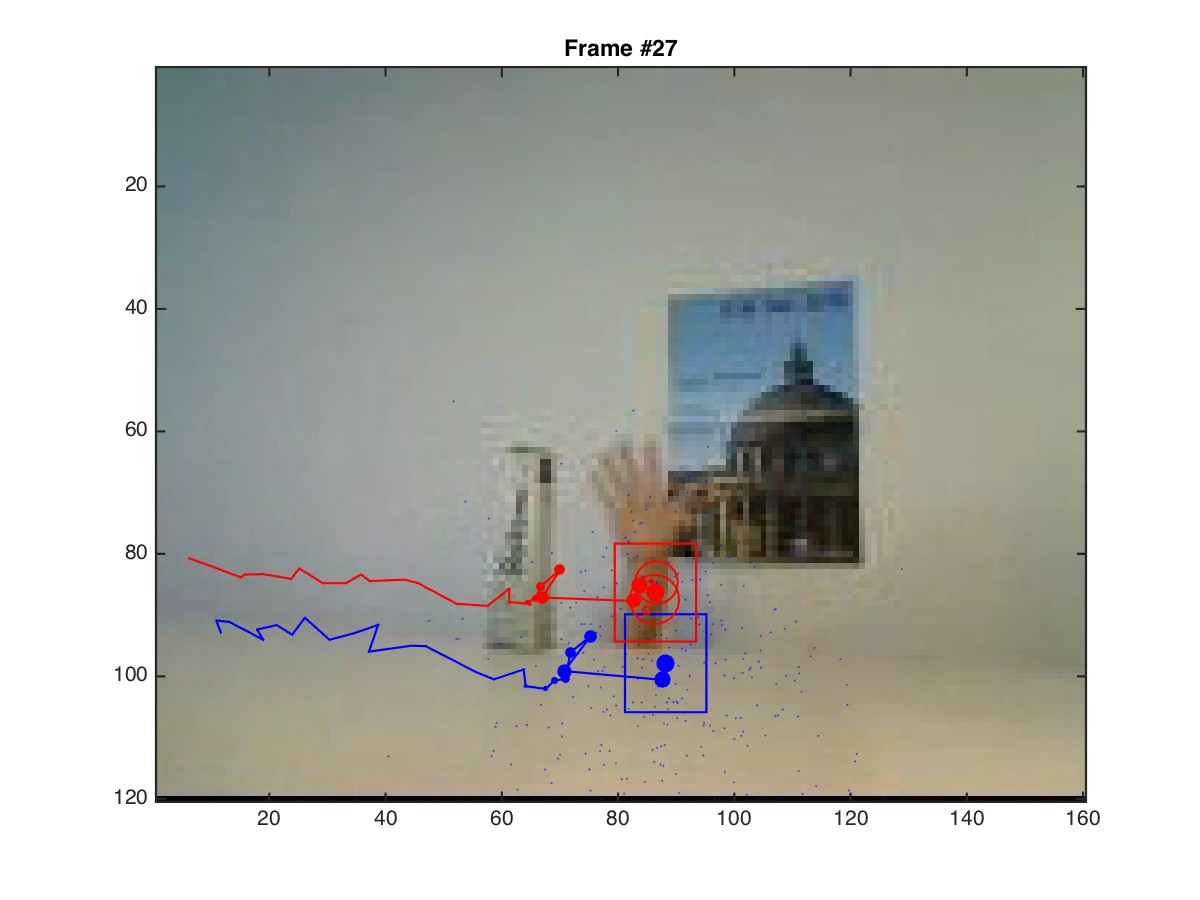
\includegraphics[width=1\linewidth]{images/video2_model_26}
    \end{subfigure}%
    \begin{subfigure}[b]{.25\textwidth}
        \centering
        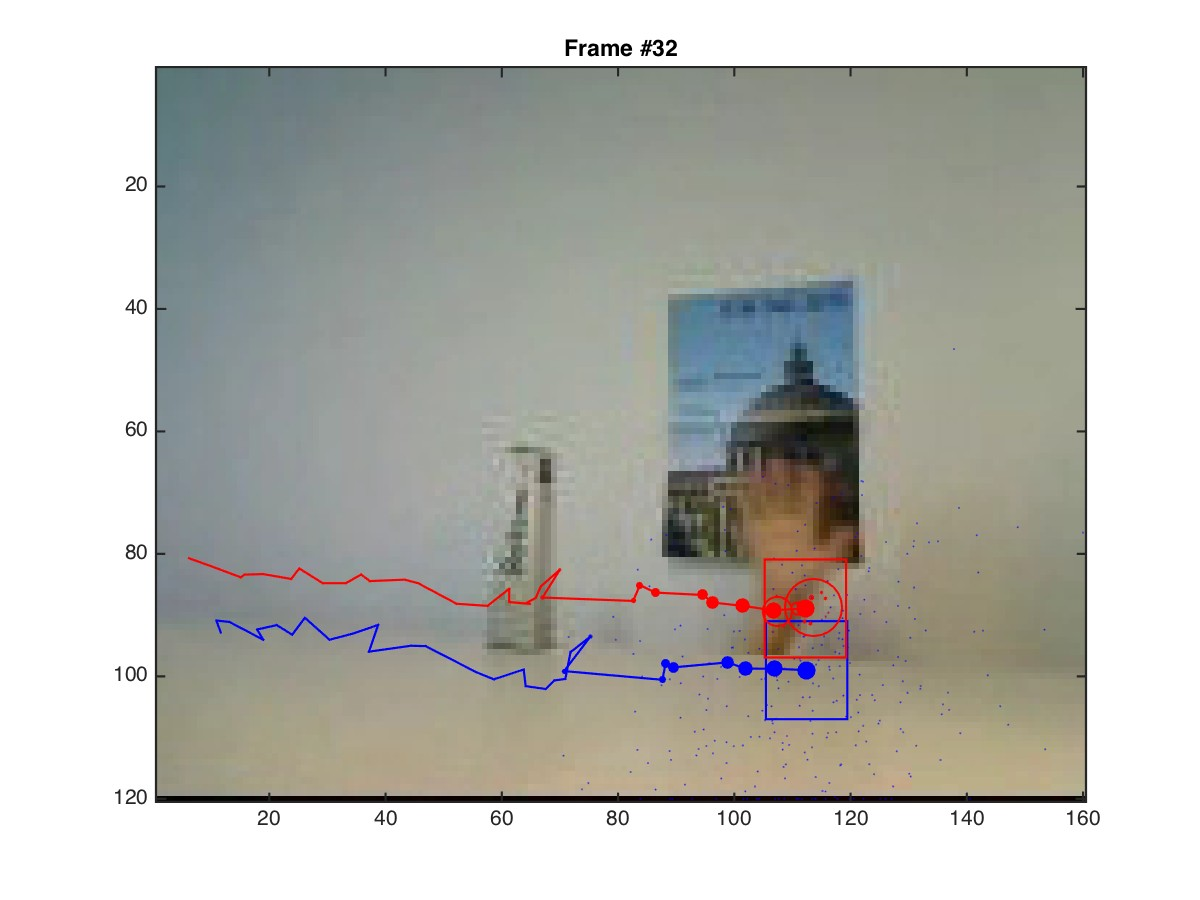
\includegraphics[width=1\linewidth]{images/video2_model_31}
    \end{subfigure}%
    \begin{subfigure}[b]{.25\textwidth}
        \centering
        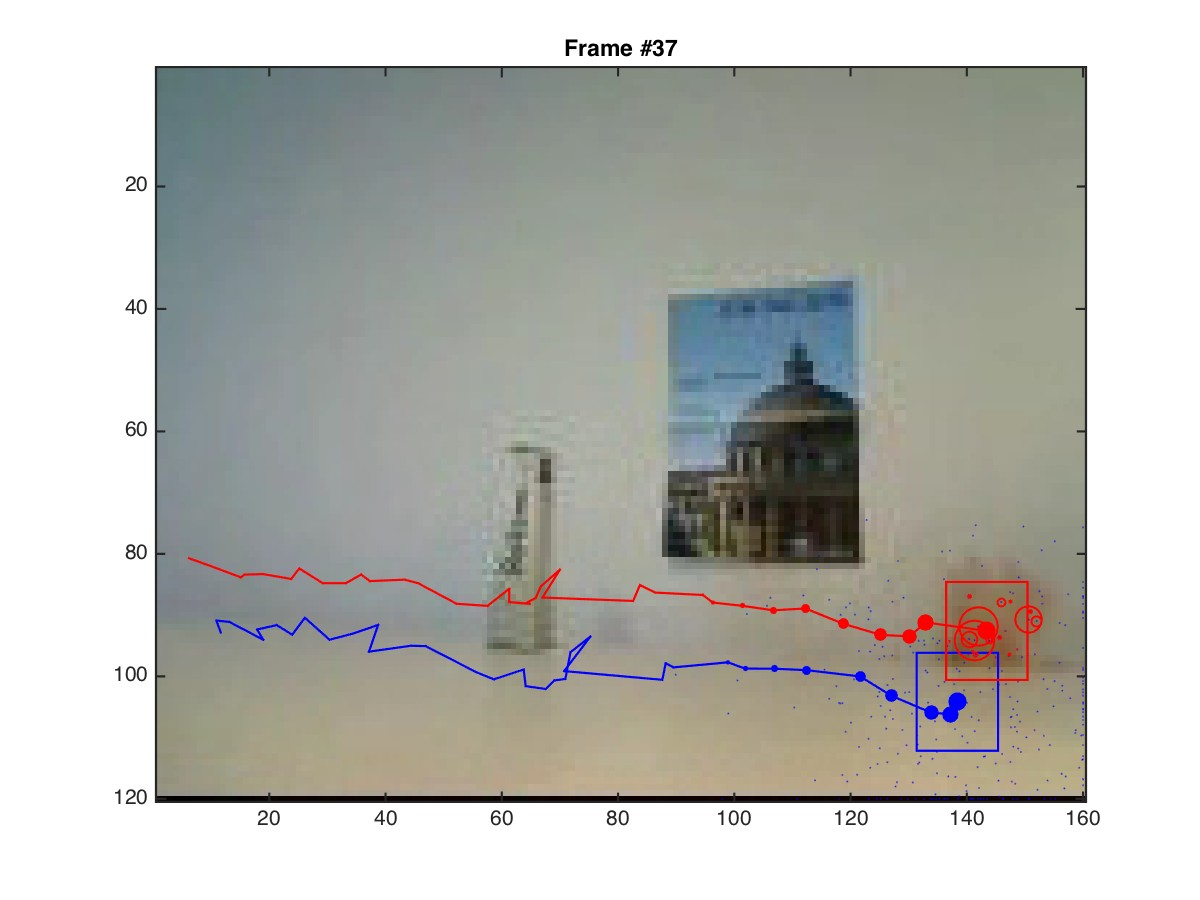
\includegraphics[width=1\linewidth]{images/video2_model_36}
    \end{subfigure}
    \caption{Tracking for the second video with the constant velocity model.}
    \label{fig:tracking_video2_model}
\end{figure}

\subsubsection*{Effect of the system noise}

\subsubsection*{Effect of the measurement noise}



\subsection*{\texttt{video3.wmv}}

\subsubsection*{Effect of the model}

\subsubsection*{Effect of the system noise}

\subsubsection*{Effect of the measurement noise}

\end{document}
